\documentclass[a4paper,11pt]{article}

\usepackage[T1]{fontenc}
\usepackage[utf8]{inputenc}
\usepackage{graphicx}
\usepackage{xcolor}

\renewcommand\familydefault{\sfdefault}
\usepackage{tgheros}
\usepackage[defaultmono]{droidmono}

\usepackage{amsmath,amssymb,amsthm,textcomp}
\usepackage{enumerate}
\usepackage{multicol}
\usepackage{tikz}

\usepackage{geometry}
\geometry{left=25mm,right=25mm,%
bindingoffset=0mm, top=20mm,bottom=20mm}

\usepackage{graphicx}
\graphicspath{ {images/} }


\linespread{1.3}

\newcommand{\linia}{\rule{\linewidth}{0.5pt}}

% custom theorems if needed
\newtheoremstyle{mytheor}
    {1ex}{1ex}{\normalfont}{0pt}{\scshape}{.}{1ex}
    {{\thmname{#1 }}{\thmnumber{#2}}{\thmnote{ (#3)}}}

\theoremstyle{mytheor}
\newtheorem{defi}{Definition}

% my own titles
\makeatletter
\renewcommand{\maketitle}{
\begin{center}
\vspace{2ex}
{\huge \textsc{\@title}}
\vspace{1ex}
\\
\linia\\
\@author \hfill \@date
\vspace{4ex}
\end{center}
}
\makeatother
%%%

% custom footers and headers
\usepackage{fancyhdr}
\pagestyle{fancy}
\lhead{}
\chead{}
\rhead{}
\lfoot{Assignment \textnumero{} 1}
\cfoot{}
\rfoot{Page \thepage}
\renewcommand{\headrulewidth}{0pt}
\renewcommand{\footrulewidth}{0pt}
%

% code listing settings
\usepackage{listings}
\lstset{
    language=Python,
    basicstyle=\ttfamily\small,
    aboveskip={1.0\baselineskip},
    belowskip={1.0\baselineskip},
    columns=fixed,
    extendedchars=true,
    breaklines=true,
    tabsize=4,
    prebreak=\raisebox{0ex}[0ex][0ex]{\ensuremath{\hookleftarrow}},
    frame=lines,
    showtabs=false,
    showspaces=false,
    showstringspaces=false,
    keywordstyle=\color[rgb]{0.627,0.126,0.941},
    commentstyle=\color[rgb]{0.133,0.545,0.133},
    stringstyle=\color[rgb]{01,0,0},
    numbers=left,
    numberstyle=\small,
    stepnumber=1,
    numbersep=10pt,
    captionpos=t,
    escapeinside={\%*}{*)}
}



\begin{document}

\title{Programming Assignment \textnumero{} 1}

\author{Juan Sebasti\'an Vinasco, Universidad del Valle}

\date{11/05/2020}

\maketitle

\section*{Problem 1}

 Follow the OTB workshop here : https://gitlab.orfeo-toolbox.org/orfeotoolbox/otb-documents/-/tree/master/Courses/org/WorkshopGuide \\ 

% code from http://rosettacode.org/wiki/Fibonacci_sequence#Python
\begin{lstlisting}[label={list:first},caption=Sample Python code -- Fibonacci sequence calculated analytically.]
from math import *

# define function 
def analytic_fibonacci(n):
  sqrt_5 = sqrt(5);
  p = (1 + sqrt_5) / 2;
  q = 1/p;
  return int( (p**n + q**n) / sqrt_5 + 0.5 )
 
# define range
for i in range(1,31):
  print analytic_fibonacci(i)
\end{lstlisting}

Following Listing~\ref{list:first}\ldots{}  \\
Lorem ipsum  \\

\section*{Problem 2}

Get a few Sentinel2 L2A product from peps (peps.cnes.fr you can create an account for free). Display them in Monteverdi, in Qgis, so as to understand what they look like, how the product are formatted \\



The objetive is understand how are constituted the format use by the data obtained from PEPS\\



\begin{lstlisting}[language=bash,caption={bash version}]
#!/bin/bash
gdalinfo S2A_MSIL1C_20200507T104031_N0209_R008_T31TDH_20200507T124549.zip 

Driver: SENTINEL2/Sentinel 2
Files: S2A_MSIL1C_20200507T104031_N0209_R008_T31TDH_20200507T124549.zip
Size is 512, 512
Coordinate System is `'
Metadata:
  CLOUD_COVERAGE_ASSESSMENT=11.0885
  DATATAKE_1_DATATAKE_SENSING_START=2020-05-07T10:40:31.024Z
  DATATAKE_1_DATATAKE_TYPE=INS-NOBS
  DATATAKE_1_ID=GS2A_20200507T104031_025459_N02.09
  DATATAKE_1_SENSING_ORBIT_DIRECTION=DESCENDING
  DATATAKE_1_SENSING_ORBIT_NUMBER=8
  DATATAKE_1_SPACECRAFT_NAME=Sentinel-2A
  DEGRADED_ANC_DATA_PERCENTAGE=0.0
  DEGRADED_MSI_DATA_PERCENTAGE=0
  FOOTPRINT=POLYGON((1.7656944498199 43.346194685301704, 3.120433646053401 43.352791985217806, 3.118527220871465 42.364010656318975, 1.785227256908992 42.35763630855867, 1.7656944498199 43.346194685301704))
  FORMAT_CORRECTNESS=PASSED
  GENERAL_QUALITY=PASSED
  GENERATION_TIME=2020-05-07T12:45:49.000000Z
  GEOMETRIC_QUALITY=PASSED
  PREVIEW_GEO_INFO=Not applicable
  PREVIEW_IMAGE_URL=Not applicable
  PROCESSING_BASELINE=02.09
  PROCESSING_LEVEL=Level-1C
  PRODUCT_START_TIME=2020-05-07T10:40:31.024Z
  PRODUCT_STOP_TIME=2020-05-07T10:40:31.024Z
  PRODUCT_TYPE=S2MSI1C
  PRODUCT_URI=S2A_MSIL1C_20200507T104031_N0209_R008_T31TDH_20200507T124549.SAFE
  QUANTIFICATION_VALUE=10000
  RADIOMETRIC_QUALITY=PASSED
  REFLECTANCE_CONVERSION_U=0.983929623995361
  SENSOR_QUALITY=PASSED
  SPECIAL_VALUE_NODATA=0
  SPECIAL_VALUE_SATURATED=65535
Subdatasets:
  SUBDATASET_1_NAME=SENTINEL2_L1C:/vsizip/S2A_MSIL1C_20200507T104031_N0209_R008_T31TDH_20200507T124549.zip/S2A_MSIL1C_20200507T104031_N0209_R008_T31TDH_20200507T124549.SAFE/MTD_MSIL1C.xml:10m:EPSG_32631
  SUBDATASET_1_DESC=Bands B2, B3, B4, B8 with 10m resolution, UTM 31N
  SUBDATASET_2_NAME=SENTINEL2_L1C:/vsizip/S2A_MSIL1C_20200507T104031_N0209_R008_T31TDH_20200507T124549.zip/S2A_MSIL1C_20200507T104031_N0209_R008_T31TDH_20200507T124549.SAFE/MTD_MSIL1C.xml:20m:EPSG_32631
  SUBDATASET_2_DESC=Bands B5, B6, B7, B8A, B11, B12 with 20m resolution, UTM 31N
  SUBDATASET_3_NAME=SENTINEL2_L1C:/vsizip/S2A_MSIL1C_20200507T104031_N0209_R008_T31TDH_20200507T124549.zip/S2A_MSIL1C_20200507T104031_N0209_R008_T31TDH_20200507T124549.SAFE/MTD_MSIL1C.xml:60m:EPSG_32631
  SUBDATASET_3_DESC=Bands B1, B9, B10 with 60m resolution, UTM 31N
  SUBDATASET_4_NAME=SENTINEL2_L1C:/vsizip/S2A_MSIL1C_20200507T104031_N0209_R008_T31TDH_20200507T124549.zip/S2A_MSIL1C_20200507T104031_N0209_R008_T31TDH_20200507T124549.SAFE/MTD_MSIL1C.xml:TCI:EPSG_32631
  SUBDATASET_4_DESC=True color image, UTM 31N
Corner Coordinates:
Upper Left  (    0.0,    0.0)
Lower Left  (    0.0,  512.0)
Upper Right (  512.0,    0.0)
Lower Right (  512.0,  512.0)
Center      (  256.0,  256.0)


\end{lstlisting}

Now the data comes from PEPS (Plataforme d'Exploitation de Produits Sentinel) this plataform provied data from Sentinel 1, 2 and 3, from Copernicus Program. Is development and operated by CNES, and acting like a mirror site of Collaboratory Earth Segment.\\

According with Olliver Hagolle existing different processing levels, the data display correspond to Level 2A, that mean a monodate ortho-rectified image expressed in BOA (Botton Of Atmosphere ) surface reflectande and incluied also cloud, shadow, snow and water mask.\\


After see the output of the command and read the documentation of PEPS \\

The firts image corresponde with Red, Green, Blue composition.\\

\begin{figure}[h]
    \centering
    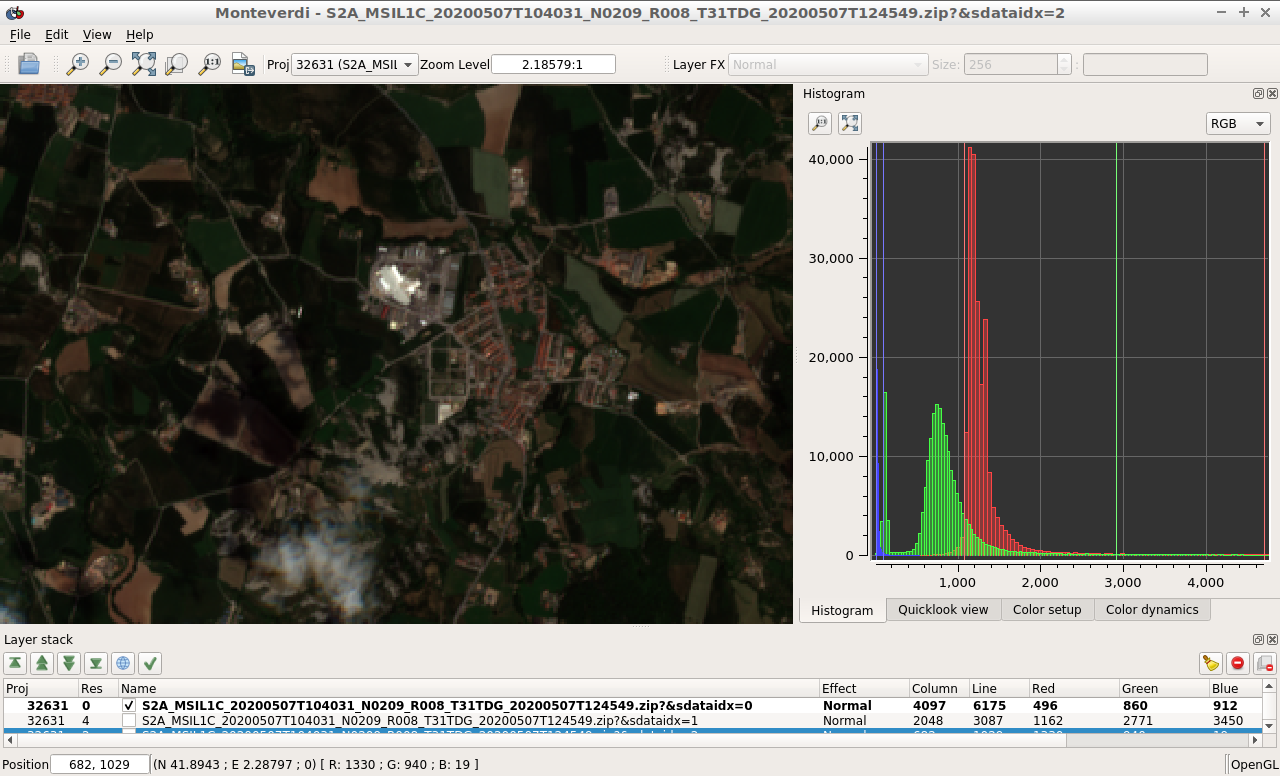
\includegraphics[width=0.8\textwidth]{displayS2A.png}
    \caption{a nice plot}
    \label{fig:mesh1}
\end{figure}

The second correspond to a index ndvi image.\\

\begin{figure}[h]
    \centering
    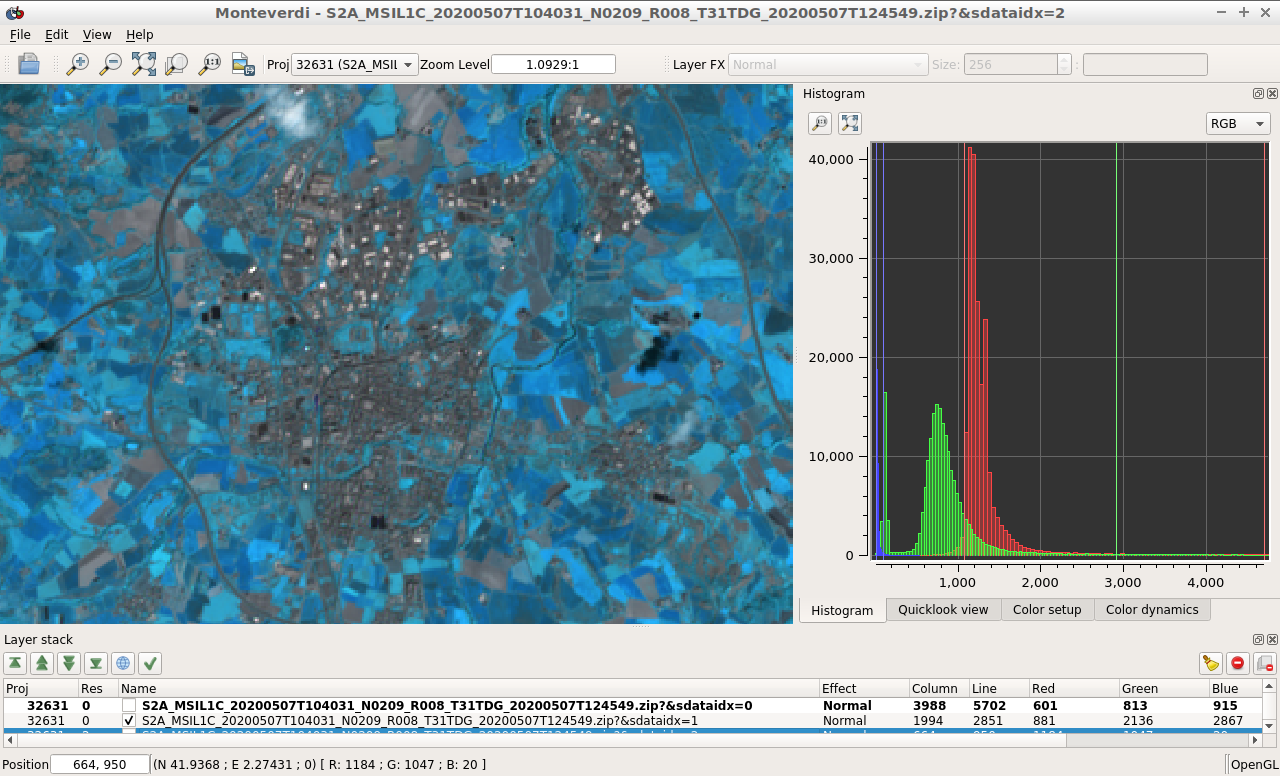
\includegraphics[width=0.8\textwidth]{displayS2A_index.png}
    \caption{a nice plot}
    \label{fig:mesh1}
\end{figure}

The third correspond to a index ndvi image.\\

\begin{figure}[h]
    \centering
    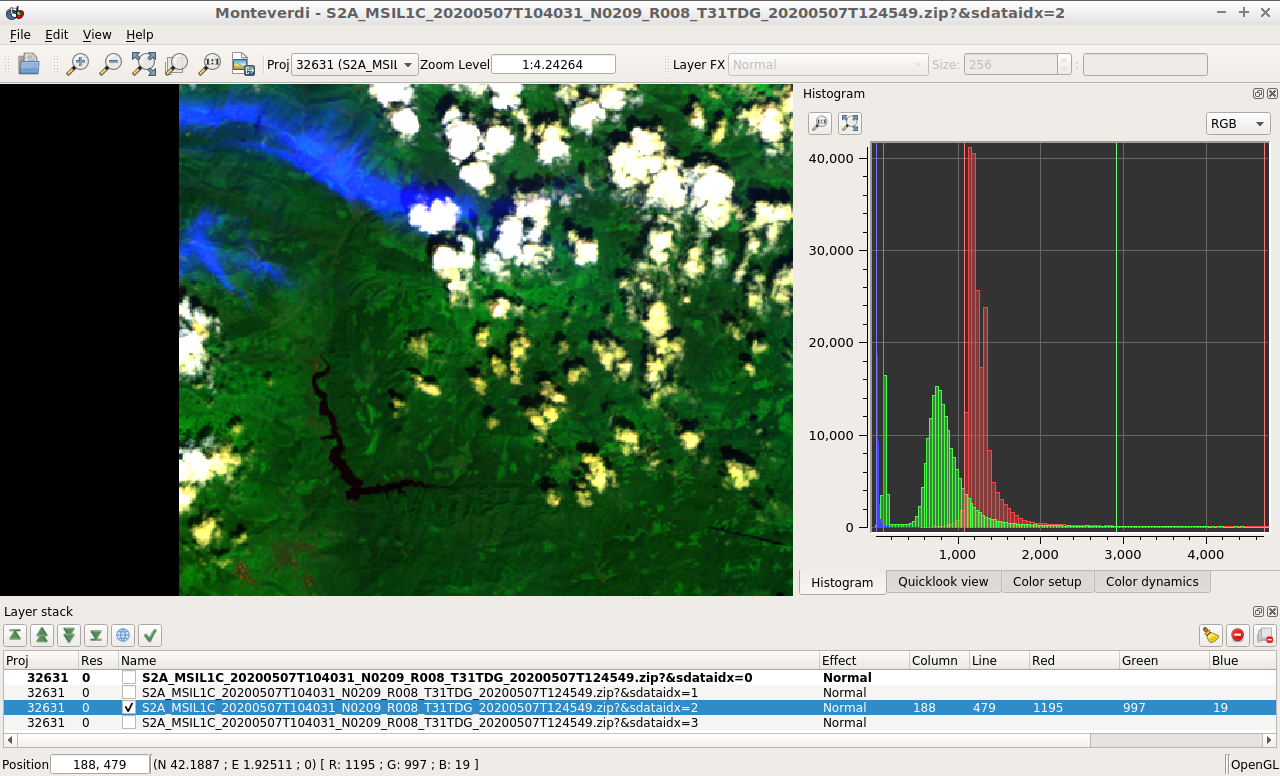
\includegraphics[width=0.8\textwidth]{displayS2A_index2.png}
    \caption{a nice plot}
    \label{fig:mesh1}
\end{figure}

Finally display a :\\

\begin{figure}[h]
    \centering
    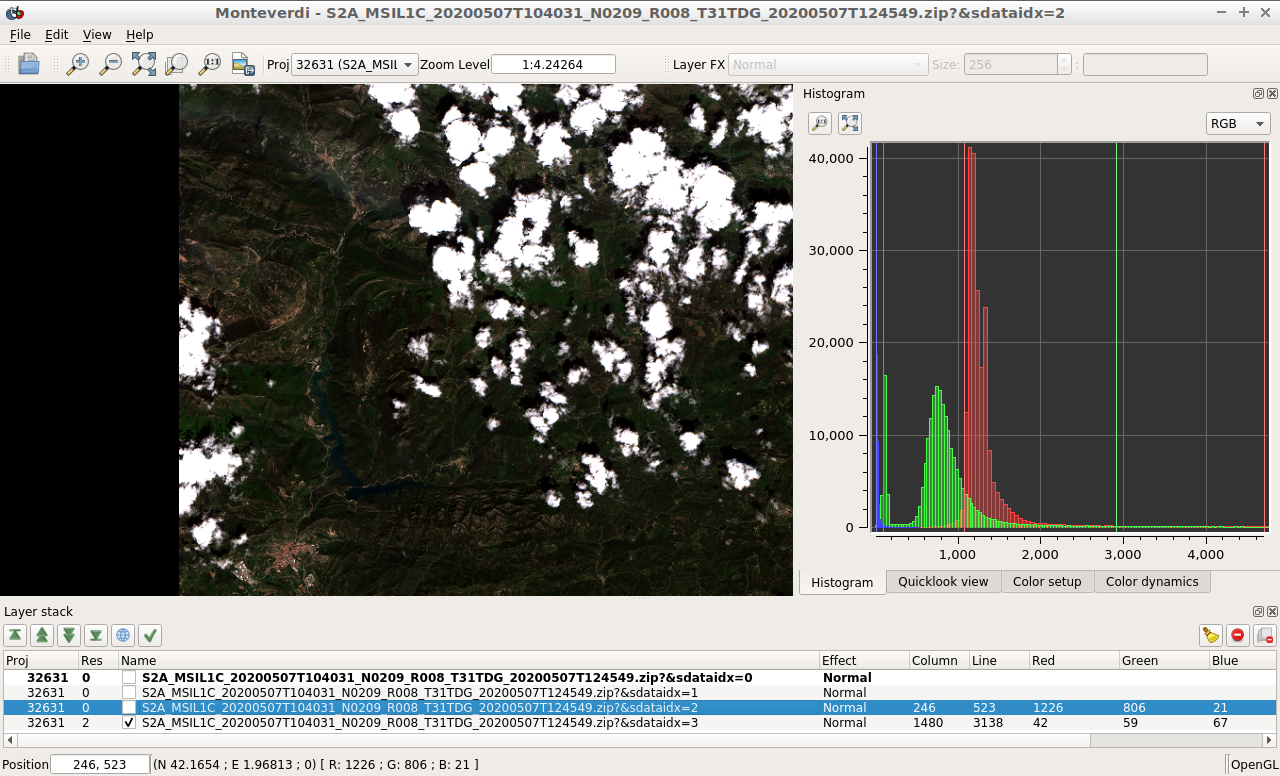
\includegraphics[width=0.8\textwidth]{displayS2A_2.png}
    \caption{a nice plot}
    \label{fig:mesh1}
\end{figure}




\section*{Problem 3}

Install rasterio (python package) and get familiar with how to read images with it, and retrieve numpy arrays. For instance write a python code that extracts a given location for all bands and then display a nice rgb image with matplotlib.\\

In the next lines I build a two examples of displaying remote sensing data, for that i use gdalinfo command for calculate the center of the image and display only a part of the image, because a limited resources of the development computer.\\


\begin{lstlisting}[label={list:first},caption=Python code -- Display Remote Sensing Images.]

# get familiar with rasterio
# import necesary librarys
import os
import numpy as np
import matplotlib.pyplot as plt
import rasterio
# define functions
# Normalize bands into 0.0 - 1.0 scale
def normalize(array):
    array_min, array_max = array.min(), array.max()
    return (array - array_min) / (array_max - array_min)
# set location of the data and code
path_code = '/home/juan/Documentos/cesbio/assigments/Code/'
path_data = '/home/juan/Documentos/cesbio/assigments/Data/PEPS/S2A_MSIL1C_20200507T104031_N0209_R008_T31TDG_20200507T124549.SAFE/GRANULE/L1C_T31TDG_A025459_20200507T104558/IMG_DATA/'
path_data2 = '/home/juan/Documentos/cesbio/assigments/Data/Venus/VENUS_20190825-151920-000_L2A_COLOMBIA_D/VE_VM01_VSC_L2VALD_COLOMBIA_20190825.DBL.DIR/'
os.chdir(path_code)
#list_img = os.listdir(path_data)
###################################
###     PART 1 PEPS SEN2 DATA   ###
###################################
# Open the file:
raster = rasterio.open(path_data+'T31TDG_20200507T104031_stack_bgr_crop.tif')
# Convert to numpy arrays
red = raster.read(3)
green = raster.read(2)
blue = raster.read(1)
# Normalize band DN
red_norm = normalize(red)
green_norm = normalize(green)
blue_norm = normalize(blue)
# Stack bands
rgb = np.dstack((red_norm, green_norm, blue_norm))
# View the color composite
plt.imshow(rgb)
#plt.show()
plt.savefig('/home/juan/Documentos/cesbio/assigments/Documento/images/PEPS_show.png')
####################################
###     PART 2 VENUS SEN2 DATA   ###
####################################
# Open the file:
raster2 = rasterio.open(path_data2+'VE_VM01_VSC_PDTIMG_L2VALD_COLOMBIA_20190825_SRE_crop.DBL.TIF')
# Convert to numpy arrays
red2 = raster2.read(3)
green2 = raster2.read(2)
blue2 = raster2.read(1)
# Normalize band DN
red_norm2 = normalize(red2)
green_norm2 = normalize(green2)
blue_norm2 = normalize(blue2)
# Stack bands
rgb2 = np.dstack((red_norm2, green_norm2, blue_norm2))
# View the color composite
plt.imshow(rgb2)
#plt.show()
plt.savefig('/home/juan/Documentos/cesbio/assigments/Documento/images/VENUS_show.png')
\end{lstlisting} 

The firt example is the Sentinel 2 Data obtain from PEPS.\\

\begin{figure}[h]
    \centering
    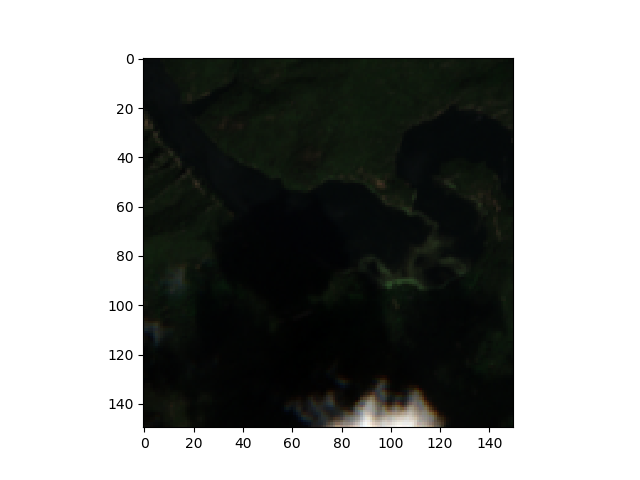
\includegraphics[width=0.8\textwidth]{PEPS_show.png}
    \caption{PEPS Sentinel 2 MSI data}
    \label{fig:mesh1}
\end{figure}

And the second is from THEIA Land for the Venus data.\\

\begin{figure}[h]
    \centering
    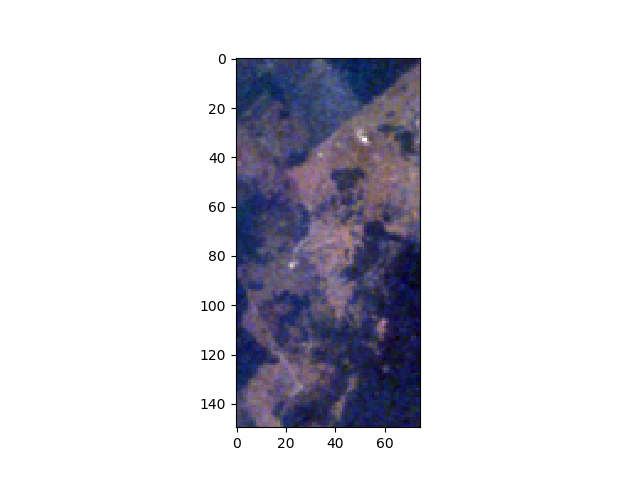
\includegraphics[width=0.8\textwidth]{VENUS_show.png}
    \caption{THEIA LAND Venus data}
    \label{fig:mesh1}
\end{figure}



\section*{Problem 4}

Install pytorch and follow one of the tutorials. T he 60 minuts  blitz is fine, but the other are interesting too (learning pytorch with examples, and What is torch.nn really?) \\


\begin{lstlisting}[label={list:first},caption=Sample Python code --PyTorch 60m blizt.]
########################################
###     Pytorch 60 minutes Tutorial  ###
########################################

# Pytorch is a library with two main funcionalities
# the firts one is a scientific computing library with GPU support
# and the second is a neuronal network library
# In the next code i follow the pytorch 60 minutes tutorial

# import the libraries

from __future__ import print_function
import torch


###################################
###     Part 1 : Torch Tensors  ###
###################################

# in the next lines is define the sintaxis 
# and behavior of the pytorch tensor 
# a replacement of numpy ndarray's

# create a matrix without initialized 
# with 5 rows and 3 columns
x = torch.empty(5, 3)
print(x)
# create a random matrix 
# with 5 rows and 3 columns
x = torch.rand(5, 3)
print(x)
# create zeros matrix 
# with 5 rows and 3 columns
x = torch.zeros(5, 3, dtype=torch.long)
print(x)
# input the data manually
x = torch.tensor([5.5, 3])
print(x)
# create zeros matrix with a double data type
# with 5 rows and 3 columns
x = x.new_ones(5, 3, dtype=torch.double)      
print(x)
# create random matrix with a float data type
# with 5 rows and 3 columns
x = torch.randn_like(x, dtype=torch.float)    
print(x)                                      
# verify the matrix size
print(x.size())
###################
#### Operations ###
###################
# sum of matrix
y = torch.rand(5, 3)
print(x + y)
print(torch.add(x, y))
# using a predefine tensor to store the result
result = torch.empty(5, 3)
torch.add(x, y, out=result)
print(result)
# adds x to y
y.add_(x)
print(y)
# slicing the tensor witha numpy like sintaxis 
print(x[:, 1])
# resizing the tensor this comand change the 
# key worth reshape for view
x = torch.randn(4, 4)
y = x.view(16)
z = x.view(-1, 8)  # the size -1 is inferred from other dimensions
print(x.size(), y.size(), z.size())
# is possibly use .item() to get the value as python number
# working for a scalar data not with tensors
x = torch.randn(1)
print(x)
print(x.item())
#####################
#### NumPy Bridge ###
#####################
# Is possibly transfor pytorch tensor 
# to numpy ndarray and vice versa
a = torch.ones(5)
print(a)
b = a.numpy()
print(b)
a.add_(1)
print(a)
print(b)

import numpy as np
a = np.ones(5)
b = torch.from_numpy(a)
np.add(a, 1, out=a)
print(a)
print(b)

# CUDA Tensors
# let us run this cell only if CUDA is available
# We will use ``torch.device`` objects to move tensors in and out of GPU
if torch.cuda.is_available():
    device = torch.device("cuda")          # a CUDA device object
    y = torch.ones_like(x, device=device)  # directly create a tensor on GPU
    x = x.to(device)                       # or just use strings ``.to("cuda")``
    z = x + y
    print(z)
    print(z.to("cpu", torch.double))       # ``.to`` can also change dtype together!

####################################
###     Part 2 : Torch Autograd  ###
####################################
#The next module is the autograd (automatic differentiation)
#this package allow the differentiation operations for the tensors
#addicionally track this operation, for the train block of a neural net
#some important comand is .requires_grad as True for start the 
#operational tracking, .backward() for compute the gradients
#.detach() to stop the tracking and prevent the computation of 
#future differention calculations, with torch.no_grad(): for 
#prevent modification of the weights of the neural net are updated
#during the prediction block, and finally the  Function atributte of
#the different functions of the pytorch library, and allow compute the
#differention.
#

# create a tensor with the tracking activate
x = torch.ones(2, 2, requires_grad=True)
print(x)
# use that tensor for a operation
y = x + 2
print(y)
# show the pointer that stores the track of operations
print(y.grad_fn)
z = y * y * 3
out = z.mean()
print(z, out)
# example of how activate o desactivate the gradient track
a = torch.randn(2, 2)
a = ((a * 3) / (a - 1))
print(a.requires_grad)
a.requires_grad_(True)
print(a.requires_grad)
b = (a * a).sum()
print(b.grad_fn)

##################
#### Gradients ###
##################
# propagate the gradients 
out.backward()
print(x.grad)
# example of propagate the gradients 
# for compute the jacobian-vector producto
x = torch.randn(3, requires_grad=True)
y = x * 2
while y.data.norm() < 1000:
    y = y * 2

print(y)


v = torch.tensor([0.1, 1.0, 0.0001], dtype=torch.float)
y.backward(v)

print(x.grad)

print(x.requires_grad)
print((x ** 2).requires_grad)

with torch.no_grad():
    print((x ** 2).requires_grad)


print(x.requires_grad)
y = x.detach()
print(y.requires_grad)
print(x.eq(y).all())





###########################################
###     Part 3 : Torch Neural Networks  ###
###########################################




###############################################
###     Part 4 : Torch Training Classifier  ###
###############################################
\end{lstlisting}


\end{document}
